\section{Guided GradCAM}

Guided GradCAM is a method created by Selvaraju et al. \cite{selvaraju2017grad} which combines both GBP and GradCAM (also created by the same authors). To explain the idea of Guided GradCAM, we have to split it into separate components.

\vspace{\baselineskip}

\textbf{Class Activation Mapping} (CAM) \cite{zhou2016learning} is an approach to localize regions responsible for a class prediction. This idea replaces the fully connected layers on the CNN with more convolutional layers and global average pooling (GAP) \cite{lin2013network}. 

\begin{figure}[h]
    \centering
    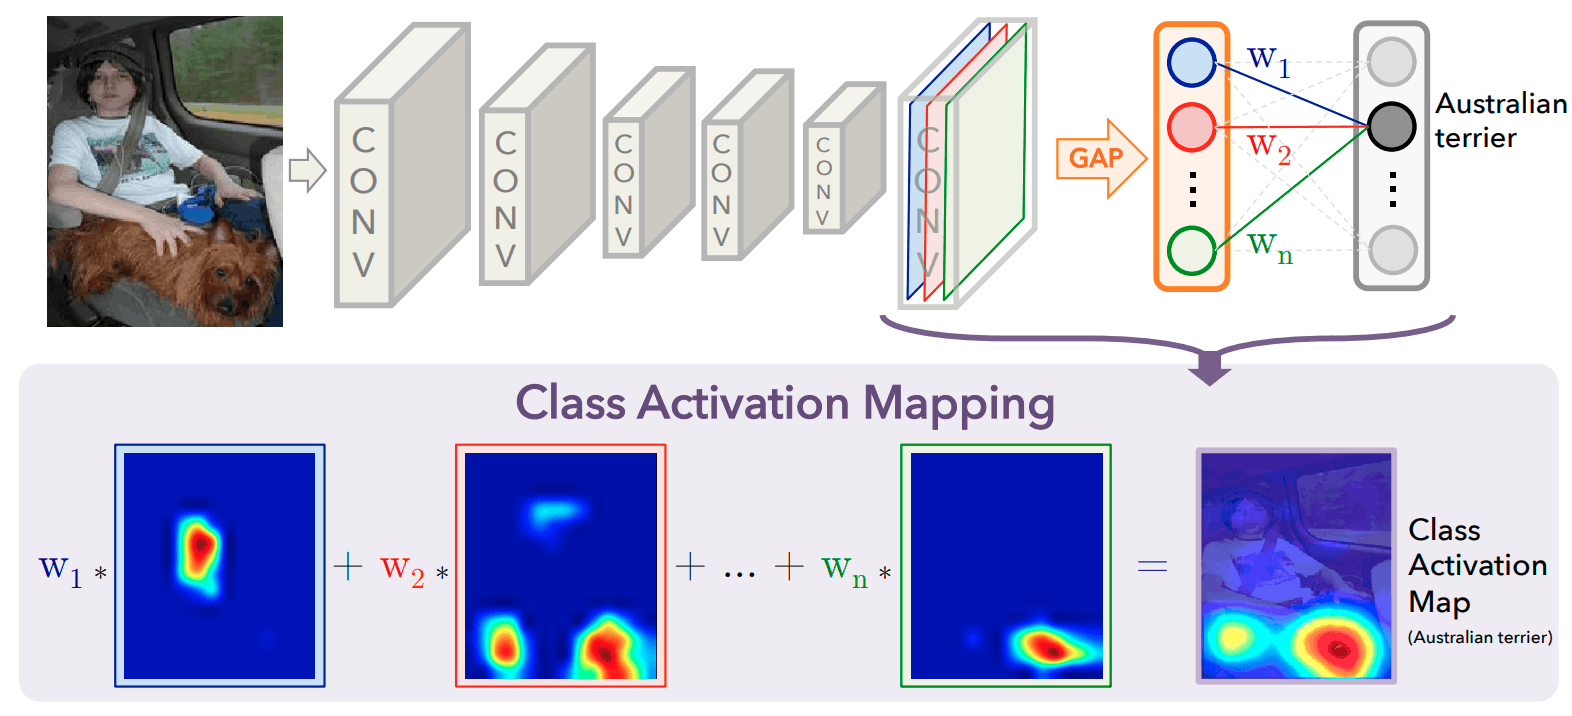
\includegraphics[width=\textwidth]{methods/images/cam-structure.png}
 \caption{The modified architecture of the CNN that produces CAMs. Source: \textit{Learning Deep Features for Discriminative Localization} \cite{lin2013network} }\label{fig:gradcam-cam}
\end{figure}

As shown in Figure \ref{fig:gradcam-cam}, just before the Softmax layer, the GAP operation is performed. This computes the spatial average of the feature map from the last CNN layer for every unit. The weighted sum of these spatial averages is calculated to produce the final output, and the Softmax layer gives us a normalized output used for classification. Class activation maps are computed similarly to the output, but the process is reversed. As an input, we have a class $c$, and the activation map for that class can be computed as:

\begin{equation}
    M_c(x,y) = \sum_{k=1}^{n} w_k^c f_k(x,y)
    \label{eq:cam-activation}
\end{equation}

Where $w_k^c$ is a weight corresponding to the unit $k$ and class $c$, and $f_k(x,y)$ is an activation of the last convolutional layer at the location $(x,y)$ for unit $k$ (visualized in Fig. \ref{fig:gradcam-cam}, the bottom part of the image).

\vspace{\baselineskip}

Selvaraju et al. argue that the CAM approach has a major drawback which is a requirement to modify the network and replace all fully-connected layers with convolutional layers. This makes CAM only applicable to certain tasks and reduces the performance of the network itself. They introduce the method that fixes all mentioned issues and call it \textbf{GradCAM}. This method is implementation agnostic (within the CNNs) and can be applied without any modifications to the network. As the name says, GradCAM uses a gradient to generate CAMs. Unlike in the original CAM paper, GradCAM allows selecting the convolutional layer we use as a feature map against which we compute the gradient. The gradient is computed for a given score $y^c$ ($c$ indicated a class) before the softmax layer. Then we use a feature map from the selected layer and calculate weight $a_k^c$ for every neuron (eq. \ref{eq:gradcam-weights}) (similar to calculating weight for every unit in CAM).

\begin{equation}
    a_k^c = \frac{1}{Z} \sum_{i} \sum_{j} \frac{\partial y^c}{\partial A_{ij}^k}
    \label{eq:gradcam-weights}
\end{equation}

\begin{figure}[ht]
    \centering
    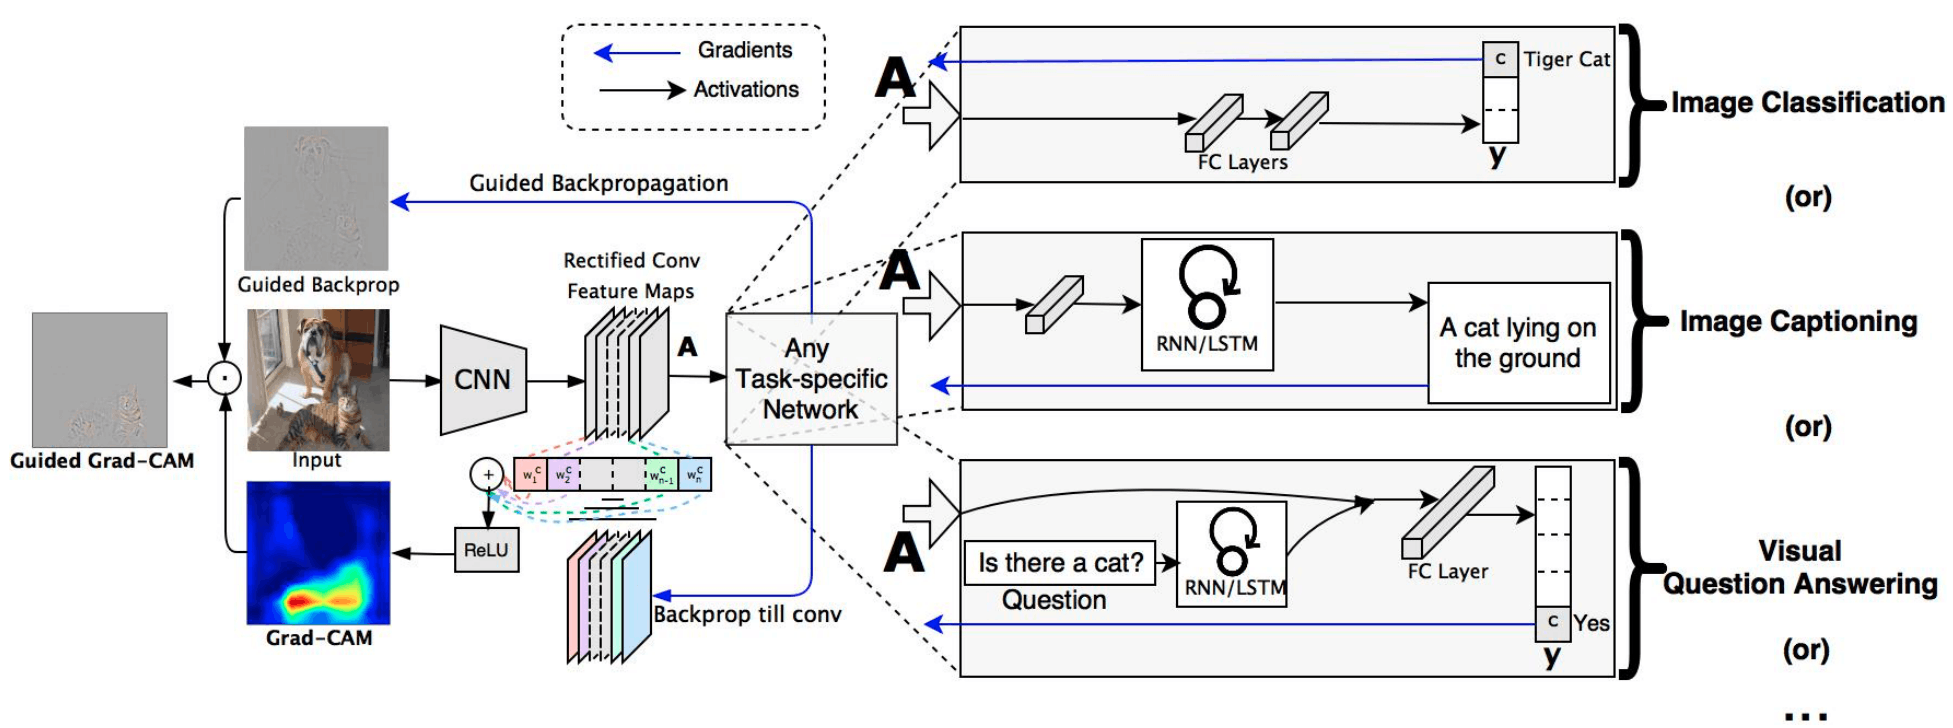
\includegraphics[width=\textwidth]{methods/images/guided-gradcam.png}
 \caption{Guided GradCAM computation process. Source: \textit{Grad-CAM: Visual Explanations from Deep Networks via Gradient-based Localization} \cite{selvaraju2017grad} }\label{fig:gradcam-guided-gradcam}
\end{figure}

$\frac{1}{Z} \sum_{i} \sum_{j}$ defines a global average pooling over the width ($i$) and height ($j$) and $\frac{\partial y^c}{\partial A_{ij}^k}$ is the gradient of score with respect to selected layers' feature map. With all $a_k^c$ calculated, we can perform a linear combination of feature maps $A^k$ and the neuron importance weights $a_k^c$ (eq. \ref{eq:gradcam-linear-combination}).

\begin{equation}
    M^c_{\text{GradCAM}} = \text{ReLU} \left(\sum_{k} a_k^c A^k \right)
    \label{eq:gradcam-linear-combination}
\end{equation}

The ReLU is used there to cutoff any non-positive values. The intuition behind using ReLU is that negative values more likely belong to other classes, which are also present in the image. The size of the map $M^c_{\text{GradCAM}}$ is the same as the size of the convolutional feature map used to compute the gradient. Values from the map then have to be mapped on the original image to visualize which region was relevant in predicting class $c$.

\begin{wrapfigure}{L}{0.50\textwidth}
  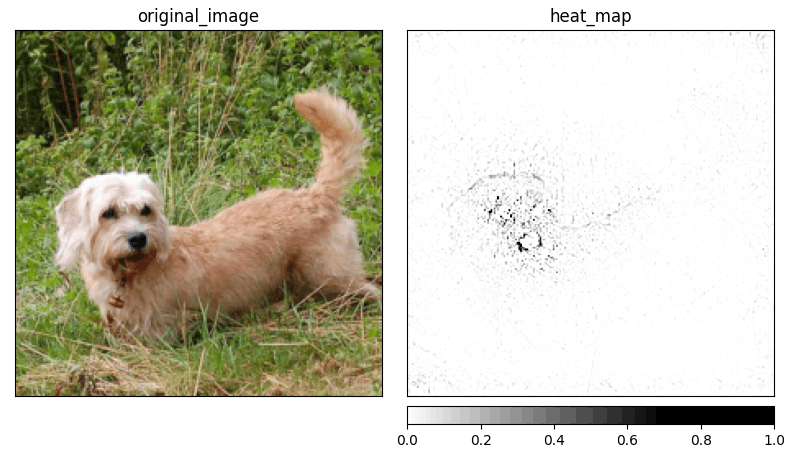
\includegraphics[width=0.50\textwidth]{methods/images/501-Dandie_Dinmont-Dandie_Dinmont.png}
  \caption{Visualization of the saliency map by the Guided GradCAM generated for the class \textit{dandie\_dinmont}. Image source: \textit{Stanford Dogs} \cite{stanford-dogs}}\label{fig:gradcam-dandie}
\end{wrapfigure}

\vspace{\baselineskip}

Guided GradCAM is a combination of GradCAM's map and GBP attribution. To compute the Guided GradCAM value, we are performing Hadamard product (also known as element-wise multiplication) of the attribution from GBP with a map from GradCAM (see Fig. \ref{fig:gradcam-guided-gradcam}). Combining GBP and GradCAM allow us to generate sharp attributions, as presented in Figure \ref{fig:gradcam-dandie}.